
\startfirstchapter{Introduction}
\label{chapter:introduction}

In recent years, advances in computer storage and processing
technology have enabled the digitization of large archives of
bioacoustic data.  Many such archives that were previously stored on
analogue magnetic tape have begun to be digitized and analyzed and
presented to the research community and public through online web
resources.  The Cornell Lab of Ornithology is one such organization,
and has recently made available a huge amount of the recordings of
birds through their website.  Here at the University of Victoria, we
have developed The Orchive, one of the largest repositories of
bioacoustic data in the world, containing over 20,000 hours of
recordings of orca vocalizations, collected from a land based research
station at Hanson Island on the BC coast.

In addition, these same advances have led to researchers becoming even
more adventerous in the collection of large amounts of bioacoustic
data, skipping the process of recording onto analog tape and recording
directly into the computer.  One of these projects is the Alberta
Biodiversity Monitoring Initiative (ABMI) which every summer records
audio from over 1700 distinct locations from the entire area of the
province of Alberta and employs researchers to annotate the recordings
based on the precense of birds in order to monitor biodiversity
changes over time.  The VENUS and NEPTUNE projects are cabled undersea
observatories that continuously record many kinds of data, including
salinity, pressure and video, and of relevance to my thesis, also
record audio data.

The amount of audio data recorded by these various projects is truly
immense, and in order for researchers to make sense of this data,
specialized tools to navigate, listen to, annotate, analyze and
classify are required.  In addition, in many cases, because of the
large amount of data traditional algorithms cannot be used to analyze
this data.  For example, one algorithm used traditionally in analyzing
audio is the Dynamic Time Warping algorithm.  In a naive
implementation, this algorithm requires $O(n^2)$ time and space
complexity, when run on small datasets, this is acceptable, but is not
when run on datasets of many thousands of hours.  In many cases, the
we must search for linear ($O(n)$) algorithms in order to make the
problem tractable, however, algorithms that exhibit constant time
performance ($O(1)$) would be even more preferable.

In order to study these complex and oft-time messy datasets, one must
use a hybrid approach that combines tools that allow for exploration
of datasets to allow for the formation of hypotheses.  

In this work, I will describe my work in applying advanced audio
feature extraction, analysis and visualization tools to a variety of
different problem domains.  These domains include the study of Orca
vocalizations and the study of bird songs.  Although these application
areas are quite different, the tools and techniques that we use to
study each of them are very similar.  There are two distinct types of
tools that will be demonstrated, the first are tools to extract
features and analyze audio.  The second set of tools are web-based and
allow users from around the world to collaboratively view and analyze
the results obtained from the first set of tools.

An aspect characterizing this work is the need to collaborate with
domain experts, and a large amount of the effort in this project is
devoted to interfaces that allow domain experts with varying degrees
of computer sophistication to access and make sense of the extracted
data that our tools produce.  Thus, the core part of this work is to
bring together tools, data and scientists together into a highly
effective collaborative team.

This work draws on ideas and concepts from many disciplines.  Because
of this it is essential to include not only definitions of these
concepts, but also the fields from which them come.  These are
presented in the Glossary chapter.

In this work I will demonstrate that I have made the following novel
contributions to the field:

1) The development of a web-based interface that allows for experts in
bioacoustics to upload, view, listen to and annotate recordings.

2) Development of a system to allow researchers to quickly and easily
build versions of a simple casual game based on a matching paradigm
that they can deploy and collect data from citizen scientists in order
to help annotate large databases.  Results are presented using a
variety of different populations of users, including in-person tests,
expert users, people of the orcalab community, tests using
undergraduate and graduate students via an emailing list, social
distribution of the game using facebook, google+ and twitter, and
users recruited through the use of Google ads.

3) Development of a system that integrates a number of different
packages for extracting audio features from recordings and to display
those features to users.  This system is highly interactive and allows
them to quickly change parameters of the algorithms and view the data
using a web-based interface.

4) Development of a system to allow for researchers in bioacoustics to
quickly and easily generate training and testing sets of data from
recordings, to train machine learning classifiers on this data, and to
run these classifiers in real-time on data.

5) Development of a system to allow researchers to run these audio
feature extraction and machine learning programs on large amounts of
data using clusters of computers, and to then view the results of
these computations in a web based interface.  This system allows for
both the use of traditional grid based resources on datasets, which
works well with a number of problems in bioacoustics that are
embarassingly parallel.  This system also integrates a map-reduce
based system to allow researchers to run

6) Testing of the effectiveness of different audio feature extraction
and machine learning algorithms on bioacoustic data, and results from
using these algorithms.  This includes the use of spectral based audio
features, such as Mel-Frequency Cepstral Coeffients (MFCC),
autocorrelation based approaches such as the Yin pitch detection
algorithm, Side-Band Interval algorithsm (SBI) and models that are
based on the human auditory cortex, specifically correllogram based
approaches.  The effectiveness of different classification algorithms
using these audio features is explored, using algorithms such as
Support Vector Machines, Self-Organized Maps, and Vector Quantization
are explored.

7) Transformation of audio features into string based representations,
and the use of tools from bioinformatics to search through these
datasets, and the results showing the benefits of using these
algorithms on bioacoustic data.


\section{Background and Motivation}

Animals and insects make a wide variety of sounds, and humans have
been interested in and studied these sounds since the time of
Aristotle \cite{aristotle} and before.  The sounds made by animals are
produced for a wide variety of purposes, from the echolocation clicks
of bats, to altering others to the presence of threats, to
communication for finding mates, and for other kinds social
interaction.  These sounds are often quite characteristic of the
species in question, and humans have long been able to identify
different animals by the sounds that they make.  

The sounds produced by animals and insects can be produced in a wide
variety of ways, and can be of a wide range of frequencies and
amplitudes.  The range of human hearing is approximately 20 Hz to
20,000 Hz, \cite{} and while many animals make sound in this range,
others, such as bats, make sound in the ultrasonic range, while others
like elephants, produce sound below the range of human hearing.  The
amplitude of sounds produced by animals is similarily diverse, with
some producing sounds inaudible to humans, while others like the blue
whale can produce sounds in excess of 188 decibels \cite{}.

Before the advent of electro-mechanical and electronic recording
devices, sounds were often described by researchers using
transliterations of animal sounds onto human speech, a simple example
is the song of the Chickadee \textit{(Poecile spp.)} which is
represented in human speech with the words ``chick-a-dee-dee'' or the
sound of the Tawny Owl \textit{(Strix aluco)} which is represented by
the words ``tu-whit tu-whoo''.  An interesting historical aside is
that in different languages, different words are used to represent the
sounds of animals, such as the ``meow'' of a cat in English, ``miaou''
in French, ``miyav'' in Turkish and ``nyan nyan'' in Japanese.

The earliest quantitative study of animal sounds began with the
recording of sounds onto wax cylinders, and the visualization of
sounds was a byproduct of the way that sound was recorded onto these
cylinders \cite{}.  The creation of permanent recordings of animal
sounds was a huge leap forward for the field of biacoustics as it
allowed researchers to record the sounds of animals and to listen to
and analyze them in more detail in a laboratory environment.  It also
allowed the scientists to distribute their recordings to other
researchers, and faciliated scientific discourse in this field.

Early devices such as the Phonoautograph of Edouard-Lyon Scott de
Martinville developed in 1857 and the Phonodiek of Dayton C. Miller
developed in 1909 allowed for the visualization of the waveforms of
sounds, and Alexander Graham Bell created a device that permanently
recorded traces of sounds onto smoked-glass.  It is relatively
difficult to analyze bioacoustic sounds purely by their waveforms, as
they are often composed of multiple overlapping harmonics, and the
relative phase of these harmonics can make sounds that sound similar
to the ear look quite different when visualized as a waveform.

In humans sounds pass through the ear canal and impact on the ear
drum, which is connected to three small bones, terminating in the
stapes (stirrup) which is connected to the oval window of the cochlea.
The cochlea is a fluid-filled spiral shaped organ which contains a
variety of structures, including the scala vestibuli, the scala
tympani and the basilar membrane.  The vibrations transmitted to the
oval window travel through the scala vestibuli and different
frequencies crest at different locations on the basilar membrane.
These vibrations move small cilia which are connected to nerves that
send electric impulses to the Medial Superior Olive, a nexus of
neurons that performs a peak triggering function similar to
autocorrelation \cite{lyon10}.  This means that the human hearing
system is sensitive to different frequencies, but is also sensitive to
the fine-timing relations of peaks in the waveform in the different
freqency bands correpsonding to place along the basilar membrane.
\cite{waltersphd}.

Because of the sensistivity of humans and other animals to the
frequencies of sounds, devices that could separate sounds into their
characteristic frequency bands proved very useful in the study of
bioacoustics sounds.  The first such commercially available device was
the Sona-Graph, produced by the Kay Electric company.  This device
produced a two-dimensional representation of sound, with frequency
along one axis and time along the other.  It had two settings for the
production of images, a narrow-band mode and a wide-band mode.  The
narrow-band mode had good frequency resolution at the expense of time
resolution, an example of this is shown in Figure
\ref{fig:sonagraph1}.  The wide band mode emphasized time resolution
at the expense of frequency resolution, an example of this is shown in
Figure \ref{fig:sonagraph2}.  The Sona-Graph was widely used in the
field of bioacoustics and was used to describe the songs of many birds
and other animals and insects.

\begin{figure}[t]
\centering
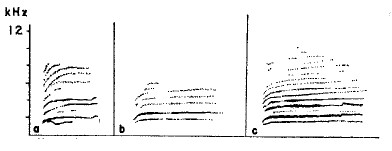
\includegraphics[width=\columnwidth]{chapter_introduction/sonagraph1}
\caption{Alarm calls of Lawrence's, Lesser, and American Goldfinches
  (\textit{Carduelis lawrencei}, \textit{Carduelis psaltria} and
  \textit{Carduelis tristis}. From Coutlee 1971, Animal Behavior
  19:559.}
\label{fig:sonagraph1}
\end{figure}

\begin{figure}[t]
\centering
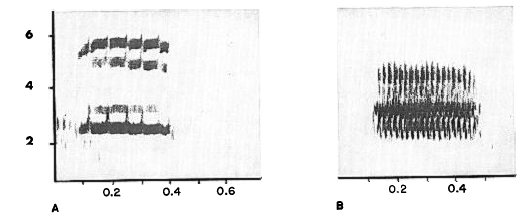
\includegraphics[width=\columnwidth]{chapter_introduction/sonagraph2}
\caption{The calls of the Varied Thrush \textit{(Ixoreus
    naevius)}. From Martin 1970, Condor 72:453.}
\label{fig:sonagraph1}
\end{figure}

While originally bioacoustic data was recorded onto wax cylinders, for
most of the 20th century, audio was recorded onto analog magnetic
tapes.  These tapes were capable of storing large amounts of data, and
allowed researchers to more easily record the sounds of animals in the
field and the lab.  Analog audio tapes were supplemented by the
introduction of Digital Audio Tapes (DAT) by Sony in 1987.  However,
one limitation of both of these forms of storage is the long time it
takes to seek to a particular place on the tape, due to the linear way
that they store data on tape.

It has only been in recent years that computer hard drives and RAM has
become able to store the large amounts of data that sound represents.
This represents another quantum leap for the field of bioacoustics, as
it allows for large amounts of audio data to be quickly accessible,
and for this data to be indexed and stored in databases and analyzed
by computers.  The field of Music Information Retrieval experienced a
similar blooming in the early 2000's, when computer storage and
computational power became great enough to store and analyze the data
of songs.  The field of bioacoustics is just starting to show similar
growth, and the use of tools from the field of Music Information
Retrieval (MIR) on bioacoustic data has shown great promise.

However, many of the tools developed for MIR are not well adapted for
the study of bioacoustic data.  When studying recorded songs, there is
often a large amount of well-curated meta-data for each song, For
example, when classifying songs based on genre, the artist, song
title, genre, record label and many other forms of data are available,
and boundaries between songs are clearly marked, and are often in
individual files.  Music often come pre-segmented into songs, which
often have identifiable sections including verse and chorus, as well
as lower level features such as beat and tatum that facilitate
analysis by computers.  In addition, most work in MIR has been on
songs that were professionally recorded in a studio environment.

In bioacoustics, this is often not the case, and in the cases of large
bioacoustic databases, recordings are often taken from a single
location, and how close animals are to the recording devices can
change dramatically during a recording.  There are often also many
sources of other sound in the recording, from environmental noise like
wind, to human produced noise like from boats or cars. Also, in many
cases there are a variety of different animals making sound in a
recording, and these sounds can overlap each other.  While some
bioacoustic recordings are well segmented, such as those of the
recordings of bird songs from the Cornell Lab of Ornithology, in many
cases of continous recordings, the locations of the bioacoustic sounds
are not localized in time, and these recordings must be annotated and
segmented before they can be analyzed.

In most studies of bioacoustics to the current time, individual
researchers record the sounds of the animals that they are interested
in studying.  In the process of doing the recording, they make notes
and record other kinds of metadata about the audio they record.  The
amount of audio that is typically analyzed is of the range of hundreds
to a few thousand recordings.  Even in larger studies such as those by
Harald Yurk on the vocalizations of Orcas, the dataset is of the order
of 1000 recordings.  These recordings are typically analyzed on a
single computer using software such as Raven \cite{ravenpro}, a
powerful tool for the study of bioacoustic data produced by the
Cornell Lab of Ornithology.  This software allows researchers to
record, import, view, analyze and annotate recordings and provides
ways to export the annotations to other programs that can be used to
further analyze the audio.  It works best with shorter audio files,
although large files can be read in and viewed using a paging
metaphor, where sections of several minutes of audio are visualized at
a time.

In recent years, the larger storage and computational capacity of
computers has inpsired researchers to analyze larger and larger
collections of bioacoustic data.  Much of the historical audio
recordings are present on audio tapes, and using high-throughput audio
digitization facilities, this data has begun to be transferred to
digital form.  At the University of Victoria, we have previously
described a project called The Orchive \cite{sness2008} where we have
digitized over 20,000 hours recordings from the Orcalab research
facility, stored originally on 45 minute long analog audio cassette
tapes.  These recordings contain large numbers of the vocalizations of
Orcas (\textit{Orcinus orca}) along with other species of marine
mammals.

Another project that collects large amounts of recordings of animals
is the Alberta Biodiversity Monitoring project (ABMI), a project setup
by the Alberta Government to monitor the biodiversity of ecosystems
across the province.  Every summer, researchers are sent to a grid of
over 1700 sites across the province, where they visually make note of
plant and animal species they encounter.  At the same time they are
doing this, they set up a stereo microphone and record 30 minutes of
audio from the site.  During the following fall and winter, a set of
researchers are employed to listen to these recordings and annotate
individual birds in the recording.  These annotations are then used to
determine the changes in biodiversity in the environment.  This
process of annotating birds is done using a simple audio visualization
tool (typically Audacity \cite{audacity}), along with a combination of
Excel spreadsheets, websites that contain examplars of birdsong of
different species, and other web based and electronic resources.

With the advent of computers that can store this large amount of data,
even more ambitious efforts have recently begun to collect continous
data including audio.  Two of these projects are the closely related
VENUS and NEPTUNE ocean observatories, part of Ocean Networks Canada.
In these projects, permanent undersea observatories that are directly
connected via cable links to land collect continous data, including
salinity, pressure, echo sound data, video and audio.  This data
streams in from 6 different observatories, and in the case of audio
data, in many of the locations, multiple channels of high sample rate
audio are collected.  This project has already collected thousands of
hours of audio, and is planned to collect data for the next 25 years.

The advent of very large bioacoustic databases of tens or hundreds of
thousands of hours presents problems to currently existing tools.
Even in the case of the 45 and 30 minute recordings from the Orchive
and ABMI projects, current tools have some issues with allowing
researchers to quickly load the audio, view it, and quickly navigate
around within and between these files.  In addition, the storage space
required for these large audio collections makes it impractical for
researchers to have the whole collection on a local computer.  In the
case of the Orchive, the entire dataset takes about 20TB of disk space
when stored as uncompressed audio files.

The MIR tools used to analyze this audio are also impractical to use
on a single computer, the time it takes to analyze the audio, and the
amount of storage space makes it impractical to analyze large
collections of audio data on a single computer.  It is also important
for researchers to be able to collaborate on these large scale
projects, to share their annotations, audio data, and the raw results
of their analysis with colleagues.  In order to do this, one possible
approach would be to use a web-based system, where the individual
researcher can connect to a large server based system that presents
the data to them in an easy to use form, allows them to make and share
annotations, and connects to large amounts of computing resources for
them to perform audio feature extraction, machine learning and other
forms of analysis on their data.
 
Web-based software has been helping connect communities of researchers
since its inception.  Recently, advances in software and in computer
power have dramatically widened its possible applications to include a
wide variety of multimedia content.  These advances have been
primarily in the business community, and the tools developed are just
starting to be used by academics. We have been working on applying
these technologies to ongoing collaborative projects that we are
involved in \cite{sness2008}. By leveraging several new technologies
including HTML5/Javascipt, Node.js and Python we have been able to
rapidly develop web-based tools.  Rapid prototyping and iterative
development have been key elements of our collaborative
strategy. Although our number of users is limited compared to other
areas of multimedia analysis and retrieval, this is to some degree
compensated by their passion and willingness to work closely with us
in developing these tools.


\subsection{Relevance of this work}

An important aspect in the design of a tool to support collaborative
work is to consider what user communities will use the tool.  In the
case of the Orchive, there are a number of different scientific
communities that will be using this tool and the data this tool
provides access to.  The primary scientific community that will
benefit from this work will be cetacean biologists.  In order to study
the rich archive orca vocalizations that have been recorded by
Orcalab, researchers must currently travel to Hanson Island, search
through the lab books and incidence reports to find which recordings
contain the data they are interested in, locate the physical cassette
tape corresponding to this recording, and then either manually listen
to the tape, or perhaps digitize the tape and analyze it in the
computer.  Each researcher typically then keeps the annotations and
data generated from this procedure themselves, if future researchers
want to obtain this data for further analysis, they must first be
aware of the fact that this researcher has the data, and then request
it from them.  With the distributed collaborative system we have
designed, not only can these biologists easily listen to any recording
in the entire archive from any internet connected computer in the
world, and compare different recordings, they can also add their
annotations to the system.  These annotations can be either private or
public, if they are for use in a publication, after the article has
been accepted for publication, the researcher can make their private
annotations public.  These researchers are less interested in the
details of audio feature extraction and machine learning algorithms,
and are instead more focused on asking biologically informed
questions, like dialect change in cetacean call repertoire
\cite{deecke00}.

Another scientific community that will receive benefits from this
archive are the developers of bioacoustic algorithms.  These
scientists are typically computer scientists with interests in Music
Information Retrieval and bioacoustics.  This archive represents a
site where researchers can get large amounts of high quality and
uniformly collected data.  Researchers interested in bioacoustic
algorithms have different goals and skill sets from cetacean
biologists, for example, many have extensive knowledge of Digital
Signal Processing and audio feature extraction algorithms.  This
system should be flexible and powerful enough to allow these
researchers to ask questions that are relevant to them.  The required
features for this group of users include allowing them to choose
different audio feature extraction algorithms, and to then take the
resulting data and run it against a variety of machine learning
algorithms in as flexible a manner as possible.

Another group of scientists that have expressed interest in the
Orchive are Environmental and Conservation scientists. A research
question particular interest is the effect of boat noise
\cite{foote04_orca_boat_noise} on cetaceans and on the marine
environment in general.  For these researchers, the data they will be
most interested in is the frequency and nature of orca vocalizations,
and the intensity and spectral characteristics of boat noise
\cite{holt09_orca_speaking_up}.  There are large differences in the
intensity and frequency content of boat noise depending on the type of
boat that creates it, speed pleasure craft often create a high pitched
noise that quickly moves away, tug boats have a lower pitched sound
and take a long time to move through an area, and cruise ships make a
loud and distinctively high pitched sound.  Analyzing the effects of
these various types of boat noise will help researchers to establish
guidelines for boat noise as it affects this sensitive population of
marine mammals \cite{doksaeter09_orca_herring_feeding}.

Another group of scientists that this work will benefit are those
studying the social organization of whale communities
\cite{bigg90_orca_genealogy}.  There have been studies that
investigate the transmission of culture in orca societies
\cite{deecke00} and have found evidence of this through the
examination of dialect change.  In a similar vein, other studies have
investigated social learning \cite{janik00_orca_social_communication}
in communities of orcas.  With a large database such as this, more of
these type of studies will be made possible in the future.

Another large and difficult problem domain that requires the skills of
researchers from many different fields is the investigation of orca
vocalizations.  The whale species \emph{Orcinus orca}, commonly known
as Killer Whales \cite{ford00_book_killer_whales}, are large toothed
whales found around the world, in places as far afield as Antarctica
and Alaska\cite{estes09_orca_alaska_decline}.  There are three
distinct types of Orcas, Transients, Residents and Offshores, each of
which have different feeding behaviours and different styles of
communication.  The vocalizations of orcas are complex and diverse,
and consist of a wide variety of vocalizations, which include
echolocation clicks, tonal whistles and pulsed calls \cite{deecke00}.

Around Vancouver Island there are two distinct communities of Orcas,
the Northern Residents, which have a range north of Campbell River,
and the Southern Residents, which spend time around Victoria.  Orcalab
is a research station located on Hanson Island, a small island up near
the top of Vancouver Island, directed by Dr. Paul Spong and Helena
Symonds and which studies the Northern Resident population of Orcas.
Orcalab has been recording Orca song for over 20 years, and has
amassed a huge archive of over 20,000 hours of audio on magnetic
cassette tapes.  In a collaboration with them, we are digitizing and
analyzing this huge and rich archive in a project called "The
Orchive".

In this paper, we will examine the combination of three components of
distributed cognition to help work on the problem of analyzing orca
vocalizations:

- Collaborative technologies to enable distributed cognition between
expert users in with potentially diverse domain knowledge

- The use of machine learning algorithms to provide technologies for
Intelligence Augmentation

- The use of large numbers of people from the general public in a
crowdsourcing methodology to mine through and annotate large databases
of information

Our goal is to create a system that enables distributed cognition
between these three facets, allowing expert users to collaborate,
giving them advanced machine learning algorithms to help them analyze
data, and in cases where datasets are enormous, using the power of
crowdsourcing to pore through large datasets.  In this paper we
describe an application of this approach to the problem of analyzing
the orca vocalizations.

The main motivation behind our work has been creating better
interfaces for interacting with the Orchive \cite{tzanetakis07} a
large archive of audio recordings of Orca vocalizations.  There are
stable resident populations of \textit{Orcinus orca} in the
northwest Pacific Ocean, and some of these populations \cite{ford00}]
are found near Hanson Island, off the north tip of Vancouver Island in
Canada. Orcalab is a research station that has been recording audio of
these Orca populations since 1972
\cite{deecke99}. They have amassed a huge archive of
more than 20,000 hours of audio recordings collected via a permanent
installation of underwater hydrophones.

Most of existing work in the automatic analysis of Orca calls has
focused on detection and classification rather than retrieval. A
real-time system with low computational requirements for the detection
of Orca vocalizations is described in \cite{Luke2010771}. Annotation
bootstrapping is a technique used to classify/segment hydrophone
recordings into three broad categories: voiceover, background, and
vocalizations \cite{ness08}. 

Our work was influenced by two publications that described different 
representations and methodologies for the classification of Orca
calls. Orca vocalizations consists of well-defined, discrete calls
with tonal signal components. They can be characterized by the pulse
rate contour of the goal which can be viewed as analogous to the pitch
contour of a speech or monophonic music signal. A method for computing 
acoustic similarity between pulse rate contours (normalized so that
they all have the same duration) using the discriminative error of a
Artificial Neural Network is described in
\cite{deecke99}. 

Dynamic time warping (DTW) is a technique for measuring the similarity
of two sequence that many vary in time. It mostly known in the context
of speech recognition \cite{sakoe78} but it has found applications in
many areas including video, motion and DNA sequence analysis. The use
of DTW to compute the similarity between two pulse rate contours in
the context of Orca calls has been explored in
\cite{brown07_orca_dtw}. In that work, a similarity matrix is
calculated containing all the DTW alignment costs between pairs of
pulse rate contours. This similarity matrix is then subsequently used
to calculate clusters which are then compared the ground truth call
labeling to assess the feasibility of call classification using this
approach.

\section{Scope of this work}

%%% REWRITE
The fields of Music Information Retrieval (MIR), Visualization and
web-based Human Computer Interaction (HCI) are each vast topics in
their own right, not to mention the application areas of
Ethnomusicology and bioacoustics.  So as to make the present work
tractable, we will focus on three very specific problems and will
apply a carefully selected subset of some of the tools in MIR,
Visualization and HCI to help us in developing solutions for these
areas.
%%% REWRITE

%%% REWRITE
In the field of the analysis of bioacoustic signals from
\textit{Orcinus Orca} vocalizations, we will use tools from MIR,
including Fast Fourier Transforms (FFT) to analyze and display
spectrograms, along with tools such as Mel-Frequency Cepstral
Coefficients (MFCC), average zero crossing rate, and spectral
centroid, along with many other such tools, to help us visualize and
analyze orca vocalizations.  We will be also using techniques from the
fields of Visualization and HCI, including the micro-macro view,
draggable panes, multi-resolution browsing, tagging and the layered
presentation of data.
%%% REWRITE

%%% REWRITE
We will use many of these same tools in the analysis of audio from
chant traditions around the world, and will in addition be using
techniques such as Fundamental Frequency Estimation and Dynamic Time
Warping.
%%% REWRITE

%%% REWRITE
In the area of the analysis of large music collections, we will use
many of the previous tools, including the FFT and MFCC coefficients to
extract features from the songs, and will primarily be using the
technique of Self-Organizing Maps to reduce the dimensionality of the
high dimension spaces created by feature extraction to two dimensions.
%%% REWRITE
